\documentclass{article}

\usepackage{amsmath,amssymb}
\usepackage{tikz}
\usepackage{pgfplots}
\usepackage{xcolor}
\usepackage[left=2.1cm,right=3.1cm,bottom=3cm,footskip=0.75cm,headsep=0.5cm]{geometry}
\usepackage{enumerate}
\usepackage{enumitem}
\usepackage{marvosym}
\usepackage{tabularx}

\usepackage{listings}
\definecolor{lightlightgray}{rgb}{0.95,0.95,0.95}
\definecolor{lila}{rgb}{0.8,0,0.8}
\definecolor{mygray}{rgb}{0.5,0.5,0.5}
\definecolor{mygreen}{rgb}{0,0.8,0.26}
\lstdefinestyle{java} {language=java}
\lstset{language=java,
	basicstyle=\ttfamily,
	keywordstyle=\color{lila},
	commentstyle=\color{lightgray},
	stringstyle=\color{mygreen}\ttfamily,
	backgroundcolor=\color{white},
	showstringspaces=false,
	numbers=left,
	numbersep=10pt,
	numberstyle=\color{mygray}\ttfamily,
	identifierstyle=\color{blue},
	xleftmargin=.1\textwidth, 
	%xrightmargin=.1\textwidth,
	escapechar=§,
}

\usepackage[utf8]{inputenc}

\renewcommand*{\arraystretch}{1.4}

\newcolumntype{L}[1]{>{\raggedright\arraybackslash}p{#1}}
\newcolumntype{R}[1]{>{\raggedleft\arraybackslash}p{#1}}
\newcolumntype{C}[1]{>{\centering\let\newline\\\arraybackslash\hspace{0pt}}m{#1}}

\newcommand{\E}{\mathbb{E}}
\DeclareMathOperator{\rk}{rk}
\DeclareMathOperator{\Var}{Var}
\DeclareMathOperator{\Cov}{Cov}

\title{\textbf{Rechnernetze, Übung 1}}
\author{\textsc{Henry Haustein}}
\date{}

\begin{document}
	\maketitle
	
	\section*{Aufgabe 1}
	\begin{enumerate}[label=(\alph*)]
		\item 5 Verbindungen: Jeder Rechner braucht genau eine Leitung zum Hub.
		\item Der erste Rechner braucht 4 Verbindungen, der nächste nur noch 3 Verbindungen, ... Insgesamt $4+3+2+1=10$ Verbindungen.
		\item Bei der Sterntopologie wird eine zusätzliche Leitung vom Rechner zum Hub benötigt, bei vollvermaschter Topologie werden 5 zusätzliche Leitungen zu jedem Rechner benötigt. Bei $n$ Rechnern werden bei Sterntopologie $n$ Leitungen gebraucht, bei vollvermaschter Topologie
		\begin{align}
			(n-1) + (n-2) + \dots + 1 = \frac{n(n-1)}{2} \notag
		\end{align}
		\item Die Entfernung: WANs verbinden Länder, während MANs nur innerhalb von Städten und LANs nur innerhalb von Gebäuden eingesetzt werden.
	\end{enumerate}

	\section*{Aufgabe 2}
	\begin{enumerate}[label=(\alph*)]
		\item Ein Dienst stellt eine Funktion bereit, das Protokoll ist eine Vereinbarung, wie mit den Daten umzugehen ist (Format, Anfrage, Antwort, Fehlerkorrektur, ...).
		\item Sicherungsschicht, Transportschicht, Vermittlungsschicht
		\item keine Verarbeitung der Daten notwendig, sondern nur weiterleiten
	\end{enumerate}

	\section*{Aufgabe 3}
	\begin{enumerate}[label=(\alph*)]
		\item Ablaufdiagramm
		\begin{center}
			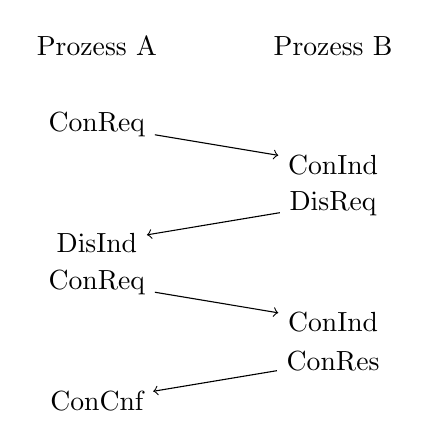
\begin{tikzpicture}
				\node at (0,1) {Prozess A};
				\node at (3,1) {Prozess B};
				
				\node at (0,0) (1) {ConReq};
				\node at (3,-0.5) (2) {ConInd};
				\node at (3,-1) (3) {DisReq};
				\node at (0,-1.5) (4) {DisInd};
				
				\draw[->] (1) -- (2);
				\draw[->] (3) -- (4);
				
				\node at (0,-2) (5) {ConReq};
				\node at (3,-2.5) (6) {ConInd};
				\node at (3,-3) (7) {ConRes};
				\node at (0,-3.5) (8) {ConCnf};
				
				\draw[->] (5) -- (6);
				\draw[->] (7) -- (8);
			\end{tikzpicture}
		\end{center}
		\item Zustandsdiagramm
		\begin{center}
			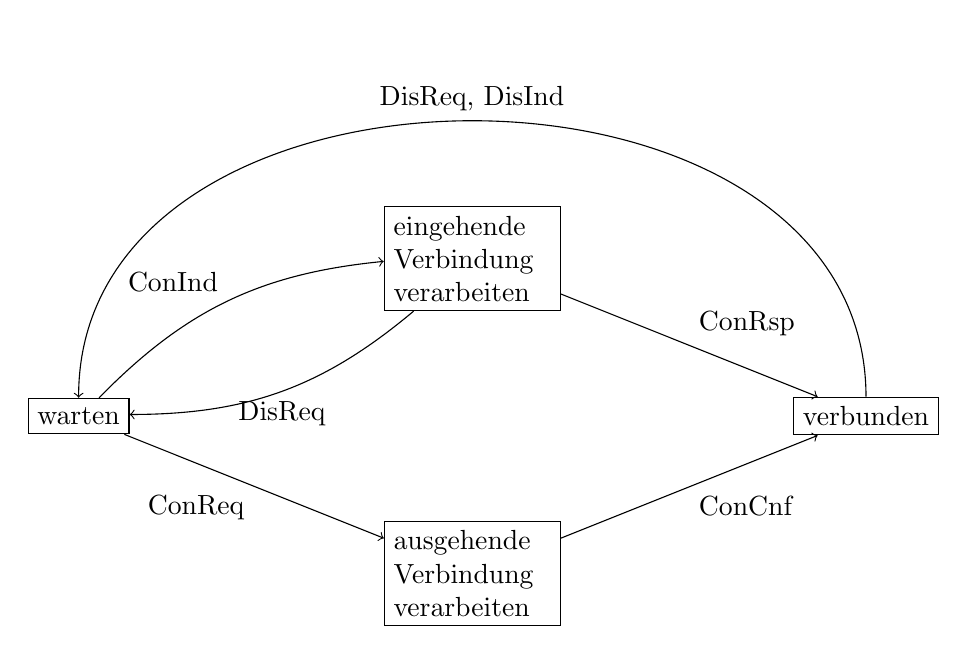
\begin{tikzpicture}
				\node[rectangle,draw=black, fill=white] (1) at (0,0) {warten};
				\node[rectangle,draw=black, fill=white, text width=2cm] (2) at (5,2) {eingehende Verbindung verarbeiten};
				\node[rectangle,draw=black, fill=white, text width=2cm] (3) at (5,-2) {ausgehende Verbindung verarbeiten};
				\node[rectangle,draw=black, fill=white] (4) at (10,0) {verbunden};
				
				\draw[->] (1) to node[below left] {ConReq} (3);
				\draw[->] (1) to[bend left=20] node[above left] {ConInd} (2);
				\draw[->] (2) to node[above right] {ConRsp} (4);
				\draw[->] (3) to node[below right] {ConCnf} (4);
				
				\draw[->] (2) to[bend left=20] node[below] {DisReq} (1);
				\draw[->] (4) to[bend right=90,looseness=1.2] node[above] {DisReq, DisInd} (1);
			\end{tikzpicture}
		\end{center}
		\item Tabelle
		\begin{center}
			\begin{tabular}{c|c|c}
				& \textbf{Ablaufdiagramm} & \textbf{Zustandsdiagramm} \\
				\hline
				Übersichtlichkeit & übersichtlich & unübersichtlich \\
				\hline
				alternative Abläufe & viele Diagramme notwendig & nur ein Diagramm notwendig \\
				\hline
				Vorlage Programmierung & nicht geeignet, weil Alternativen fehlen & geeignet
			\end{tabular}
		\end{center}
	\end{enumerate}

	
	\section*{Aufgabe 4}
	\begin{enumerate}[label=(\alph*)]
		\item Die IDU besteht aus SDU und ICI und wird an darunterliegende Schicht gegeben. In dieser Schicht wird dann aus SDU und Headern die PDU.
		\item SDU: \texttt{GET /tools/ HTTP/1.1, Host: www.heise.de} \\
		IDU: \texttt{193.99.144.85:80, GET /tools/ HTTP/1.1, Host: www.heise.de} \\
		PDU: \texttt{Src: 80, Dest: 80, Seq: 223320943, Ack: 33277, ..., GET /tools/ HTTP/1.1, Host: www.heise.de}
		\item Die Rate $b_{goodput}$ ist:
		\begin{align}
			b_{goodput} &= 125 \text{ Mbit/s} \cdot \bar{\eta}_1 \cdot \bar{\eta}_2 \cdot \bar{\eta}_3 \cdot \bar{\eta}_4 \notag \\
			&= 125 \text{ Mbit/s} \cdot 0.8 \cdot \frac{0.55+0.98}{2} \cdot \frac{0.57+0.99}{2} \cdot \frac{0.23+0.99}{2} \notag \\
			&= 36.3987 \text{ Mbit/s} \notag
		\end{align}
		bzw.
		\begin{align}
			b_{goodput} &= 125 \text{ Mbit/s} \cdot \bar{\eta}_1 \cdot \bar{\eta}_2 \cdot \bar{\eta}_4 \notag \\
			&= 125 \text{ Mbit/s} \cdot 0.8 \cdot \frac{0.55+0.98}{2} \cdot \frac{0.23+0.99}{2} \notag \\
			&= 46.665 \text{ Mbit/s} \notag
		\end{align}
	\end{enumerate}
	
\end{document}